\documentclass[11pt,answers]{exam}
\usepackage[spanish]{babel}
\usepackage[utf8]{inputenx}
\usepackage{fontenc}
\usepackage{textcomp}
\usepackage{lmodern,pifont}
\usepackage{graphicx}
\graphicspath{ {./img_/} }
\usepackage{setspace}
\usepackage[dvipsnames]{color}
\usepackage{colortbl}
\usepackage{caption}
\usepackage{amsmath}
\usepackage[normalem]{ulem}

\newcommand\titexam[1]{\centering%
\fbox{\parbox{\textwidth}{\huge \sffamily \textbf{#1}}}\normalsize \vspace{1em}}

\newcommand\materia[1]{%
\parbox{\textwidth}{ \Large \sffamily \textbf{\uline{#1}}}\vspace{1em}}


\newcommand\nombrefecha{%
Nombre y apellidos:\hrulefill
Fecha:\rule{3.5cm}{0.4pt}\vspace{0.5em}}

\renewcommand{\solutiontitle}{\noindent\textbf{Solución:}\par\noindent}
\pagestyle{empty}
\begin{document}
{\fontfamily{lmss}\selectfont

  %%%%%%%%%%%%%%%%%%%%%%%%%%%%%%%%%%%%%
  %% 
\titexam{MF1479\_2 Propagación de plantas en vivero}

\materia{Aspectos básicos de botánica y ecofisiología vegetal}

\nombrefecha
\begin{questions}
\question El nombre científico de una especie se forma de dos partes. ¿Puedes
indicar a que categoría taxonómica corresponde la primera parte?
\begin{checkboxes}
  \choice A. Al Reino
  \choice B. A la Família
  \CorrectChoice C. Al Género
  \choice D. Ninguna es correcta
\end{checkboxes}

\question ¿Sabes que terminación han de tener los taxones pertenecientes a la
categoría de la familia?
\begin{checkboxes}
  \CorrectChoice A. -aceae
  \choice B. -phyta
  \choice C. -ota
  \choice D. La categoría de familia no necesita terminación
\end{checkboxes}

\question Señala cuale de las siguientes especies son coníferas
\begin{checkboxes}
  \choice A. Plataneros, encinas y robles
  \choice B. Pinos, cedros y abetos
  \choice C. Enebros, sabinas y cipreses
  \CorrectChoice D. Las respuestas B y C son correctas
\end{checkboxes}

\question ¿En que categoría generalmente están las plantas que al frotar sus
  hojas, estas desprenden un agradable olor?
  \begin{checkboxes}
    \choice A. Plantas olorosas
    \CorrectChoice B. Plantas aromáticas
    \choice C. Plantas perfumadas
    \choice D. Plantas de rosa
  \end{checkboxes}

\question ¿Qué ecosistemas son extremadamente sensibles a la contaminación por
  plantas invasoras y con las que hay que hay que extremar precauciones?
  \begin{checkboxes}
    \choice A. Ecosistemas de montaña
    \CorrectChoice B. Ecosistemas ede agua dulce (rios y sus
    riveras, lagos, humedales, etc)
    \choice C. Ecosistemas dunares
    \choice D. Ecosistema forestal
  \end{checkboxes}
\newpage
\question ¿Qué tipo de raíz aparece en la imagen?
  \begin{figure}[h!]
    \centering
    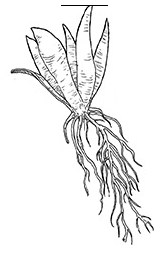
\includegraphics[width=0.2\textwidth]{fasciculada.PNG}
  \end{figure}
  \begin{checkboxes}
    \choice A. Napiforme
    \choice B. Pivotante
    \choice C. Ramificada
    \CorrectChoice D. Fasciculada
  \end{checkboxes}

\question ¿Como se llama la parte del tallo a partir de la cual se pueden
  desarrollar flores o tallos?
  \begin{checkboxes}
    \CorrectChoice A. Yemas
    \choice B. Nudos
    \choice C. Lenticelas
    \choice D. Ninguna respuesta es correcta
  \end{checkboxes}

\question ¿Como se llama la parte que une la hoja con el tallo?
  \begin{checkboxes}
    \choice A. Lamina o limbo
    \choice B. Yema axilar
    \CorrectChoice C. Peciolo
    \choice D. Nervadura
  \end{checkboxes}

\question ¿Como se llama la parte de la flor donde se forma y almacena el polen?
  \begin{checkboxes}
    \choice A. Caliz
    \CorrectChoice B. Estambre
    \choice C. Tubo polínico
    \choice D. Gineceo
  \end{checkboxes}

\question ¿Cuales son los factores ambientales que influyen en el desarrollo de
  cultivos?
  \begin{checkboxes}
    \CorrectChoice A. Temperatura, radiación e iluminación, altitud, precipitación,
    velocidad del viento
    \choice B. Topografía, orientación, climatología, frio, calor
    \choice C. Temperatura, iluminación
    \choice D. Altitud y precipitaciones
  \end{checkboxes}
\end{questions}
%%%%%%%%%%%%%%%%%%%%%%%%%%%%%%%%%%%%%%%%%%%%%%%%%%%%%%%%%%%%%%%%%%%%%%%%%%%%%%%%%%%%%%%%%%
%%%   PREGUNTAS TEMA 2 %%%%%%%%%%%%%%%%%%%%%%%%%%%%%%%%%%%%%%%%%%%%%%%%%%%%%%%%%%%%%%%%%%%

\titexam{MF1479\_2 Propagación de plantas en vivero}
\materia{Preparación del medio de cultivo}
\nombrefecha

\begin{questions}
\question ¿Cuales son los principales componentes del suelo?
  \begin{checkboxes}
    \choice A. Carbono, nitrógeno y Potasio
    \choice B. Arcilla, arena y limo
    \CorrectChoice C. Minerales de la roca madre, materia orgánica, organismos
    vivos, agua y aire
    \choice D. Roca y organismos vivos
  \end{checkboxes}

\question ¿Como se llaman las capas en las que se divide el suelo para su estudio?
  \begin{checkboxes}
    \CorrectChoice A. Horizontes
    \choice B. Franjas
    \choice C. Capas horizontales
    \choice D. Fronteras
  \end{checkboxes}

\question ¿Qué propiedad física del suelo depende del tamaño de las partículas que la
  componen?
  \begin{checkboxes}
    \CorrectChoice A. Textura
    \choice B. Porosidad
    \choice C. Estructura
    \choice D. Ninguna respuesta es correcta
  \end{checkboxes}

\question ¿Las propiedades del suelo las podemos dividir en?
  \begin{checkboxes}
    \choice A. Físicas, químicas y texturales
    \CorrectChoice B. Físicas, químicas y biológicas
    \choice C. Ph, conductividad eléctrica y capacidad de intercambio catiónico
    \choice D. Las respuestas A y C son correctas
  \end{checkboxes}

\question Los nutrientes de un suelo se clasifican en macroelementos y microelementos. ¿A
  qué se debe el nombre de estos últimos?
  \begin{checkboxes}
    \choice A. A qué la mayoría de elementos son de pequeño tamaño
    \choice B. A qué tienen poca importancia para las plantas
    \choice C. A qué se encuentran en el suelo en poca cantidad
    \CorrectChoice D. A qué se encuentran en las plantas en poca cantidad 
  \end{checkboxes}

\question El objetivo principal de la preparación de suelos es provocar transformaciones
  que mejoren la germinación y el desarrollo de las plantas. ¿Las preparaciones que se
  realizan pueden conseguir fines como?
  \begin{checkboxes}
    \choice A. Aireación del suelo y/o destrucción de hierbas no deseadas
    \choice B. Aportaciones de nutrientes o enmiendas para mejorar la calidad del suelo
    \choice C. Eliminación de actividad microbiana
    \CorrectChoice D. Las respuestas A y B son correctas
  \end{checkboxes}
\newpage
\question Las fertilizaciones en un suelo pueden ser minerales u orgánicas. ¿Qué tipo
  de fertilizantes se emplean en la fertilización orgánica?
  \begin{checkboxes}
    \choice A. Estiércol, humus de lombriz o NPK inorgánico
    \choice B. Abono verde  o enmiendas calizas
    \CorrectChoice C. Estiércol, humus, compost, guano, gallinaza, abono verde
    \choice D. Las respuestas A y B son correctas
  \end{checkboxes}


\question Cuando un suelo se encuentra bajo condiciones de exceso de agua
  permanentes y que ponen en peligro los futuros cultivos, ¿qué tipo de
  técnicas se pueden realizar?
  \begin{checkboxes}
    \choice A. Labrado profundo
    \CorrectChoice B. Drenajes
    \choice C. Escardas
    \choice D. Ninguna respuesta es correcta
  \end{checkboxes}

\question La frase: \emph{``La ropa de trabajo corriente es un EPI fundamental''}, ¿es?
  \begin{checkboxes}
    \CorrectChoice A. Falsa
    \choice B. Falsa. Solo es un EPI fundamental si los pantalones son largos
    \choice C. Verdadera
    \choice D. Verdadera solo si el operario la utiliza correctamente
  \end{checkboxes}

\question ¿Los tipos de riesgos que un operario corre por  realizar tareas de abonado del
  terreno pueden ser?
  \begin{checkboxes}
    \choice A. Sobreesfuerzos por manipular cargas o posturas inadecuadas
    \choice B. Contacto con agentes químicos o ingestión accidental de tóxicos
    \choice C. Lesiones en la piel por salpicaduras de residuos o agentes químicos
    \CorrectChoice D. Todas las respuestas son correctas
  \end{checkboxes}
\end{questions}
%%%%%%%%%%%%%%%%%%%%%%%%%%%%%%%%%%%%%%%%%%%%%%%%%%%%%%%%%%%%%%%%%%%%%%%%%%%%%%%%%%%%%%%%%%
%%%   PREGUNTAS TEMA 3 %%%%%%%%%%%%%%%%%%%%%%%%%%%%%%%%%%%%%%%%%%%%%%%%%%%%%%%%%%%%%%%%%%%
\titexam{MF1479\_2 Propagación de plantas en vivero}

\materia{Reproducción de plantas por semillas}

\nombrefecha

}
\end{document}
%%% Local Variables:
%%% mode: latex
%%% TeX-master: t
%%% End:
